% This document was generated by an LLM.

\documentclass{essay}

\usepackage{graphicx}

\title{The Infinite Power Tower}
\subtitle{Fixed Points, Stability, and the Lambert \(W\) Function}
\author{}
\date{}

\begin{document}

\maketitle

\begin{abstract}
  \noindent The expression
  \[
    x^{x^{x^{x^{\cdots}}}}
  \]
  looks self-similar, so it is tempting to replace the whole tower by a
  number \(y\) and immediately write \(y=x^y\). That equation is important,
  but it is not the definition of the infinite tower. The actual tower is a
  limit of finite towers, and the central question is whether the associated
  fixed-point iteration converges. This essay separates those two ideas:
  first solve the fixed-point equation, then ask whether the iteration is
  stable enough to reach that fixed point.
\end{abstract}

\section{Finite towers and the limiting question}

For a positive real number \(x\), define the finite right-associated towers by
\[
  a_1=x,\qquad a_{n+1}=x^{a_n}.
\]
Thus
\[
  a_2=x^x,\qquad
  a_3=x^{x^x},\qquad
  a_4=x^{x^{x^x}},
\]
and so on. The infinite power tower, if it exists, is the limit
\[
  \lim_{n\to\infty} a_n.
\]
This recurrence is the definition. The formal expression
\[
  x^{x^{x^{x^{\cdots}}}}
\]
is only a compact way of gesturing toward that limiting process.

If the sequence \(a_n\) converges to some limit \(y\), then continuity of
\(t\mapsto x^t\) gives
\[
  y=\lim_{n\to\infty}a_{n+1}
   =\lim_{n\to\infty}x^{a_n}
   =x^y.
\]
So every convergent tower gives a solution of the fixed-point equation
\[
  y=x^y.
\]
The converse is the trap: a solution of \(y=x^y\) is only a candidate limit.
It does not by itself prove that the recurrence \(a_{n+1}=x^{a_n}\) actually
settles down to that value.

\section{Solving the fixed-point equation}

The fixed-point equation is easiest to understand by solving for \(x\) in
terms of \(y\). If \(y=x^y\), then taking the \(y\)-th root gives
\[
  x=y^{1/y}.
\]
This parametrizes all positive real fixed points: choose \(y>0\), set
\[
  x=y^{1/y},
\]
and then \(y=x^y\).

The graph of \(x=y^{1/y}\) already explains the familiar upper bound. Since
\[
  \log x=\frac{\log y}{y},
\]
the function \(y^{1/y}\) reaches its maximum when
\[
  \frac{d}{dy}\left(\frac{\log y}{y}\right)
  =\frac{1-\log y}{y^2}
  =0,
\]
namely at \(y=e\). The maximum value is therefore
\[
  e^{1/e}.
\]
For \(x>e^{1/e}\), there is no positive real solution of \(y=x^y\). In that
case the tower cannot possibly converge to a positive real limit.

For \(0<x\le e^{1/e}\), fixed points do exist. But existence is still not
enough. We must ask which fixed points are stable under the iteration
\[
  a_{n+1}=f(a_n),\qquad f(t)=x^t.
\]

\section{Stability of the fixed point}

Fixed-point iteration is locally controlled by the derivative of the iteration
function. Here
\[
  f(t)=x^t,\qquad f'(t)=x^t\log x.
\]
At a fixed point \(y=x^y\), this becomes
\[
  f'(y)=y\log x.
\]
Using \(x=y^{1/y}\), we also have
\[
  \log x=\frac{\log y}{y},
\]
so the derivative at the fixed point simplifies to
\[
  f'(y)=\log y.
\]

This is the key calculation. A fixed point is attracting when
\[
  |f'(y)|<1,
\]
so here the attracting condition is
\[
  |\log y|<1.
\]
Equivalently,
\[
  -1<\log y<1,
\]
or
\[
  \frac1e<y<e.
\]
The neutral endpoint cases are
\[
  y=\frac1e\qquad\text{and}\qquad y=e,
\]
where the derivative has absolute value \(1\). Outside this interval, the
fixed point is repelling: nearby errors are not shrunk by the iteration.

\begin{figure}[ht]
  \centering
  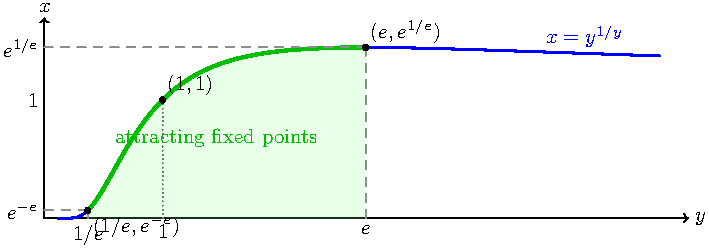
\includegraphics[width=0.82\linewidth]{power_tower_range.pdf}
  \caption{The fixed-point equation \(y=x^y\) is equivalent to
  \(x=y^{1/y}\). The attracting part of the fixed-point curve occurs for
  \(1/e\le y\le e\), giving the convergence interval
  \(e^{-e}\le x\le e^{1/e}\).}
\end{figure}

\section{The convergence interval}

The stability calculation gives the natural interval. Map the stable
\(y\)-values
\[
  \frac1e\le y\le e
\]
through \(x=y^{1/y}\). At the lower endpoint,
\[
  x=\left(\frac1e\right)^e=e^{-e}.
\]
At the upper endpoint,
\[
  x=e^{1/e}.
\]
Thus the convergence interval is
\[
  e^{-e}\le x\le e^{1/e}.
\]

\begin{theorem}
  For \(x>0\), the sequence
  \[
    a_1=x,\qquad a_{n+1}=x^{a_n}
  \]
  converges if and only if
  \[
    e^{-e}\le x\le e^{1/e}.
  \]
  When it converges, its limit is the attracting fixed point \(y\) satisfying
  \(y=x^y\).
\end{theorem}

\begin{proof}[Proof sketch]
  If the sequence converges to \(y\), then \(y=x^y\). Hence
  \(x=y^{1/y}\), and the possible fixed points are read from the graph of
  \(y^{1/y}\). Local stability of the iteration \(f(t)=x^t\) is determined by
  \[
    f'(y)=\log y
  \]
  at a fixed point. The condition \(|\log y|<1\) gives
  \(1/e<y<e\), and mapping this interval through \(x=y^{1/y}\) gives
  \(e^{-e}<x<e^{1/e}\).

  The endpoint cases \(y=1/e\) and \(y=e\) are neutral rather than strictly
  attracting, so the derivative test alone does not prove convergence there.
  A more careful monotonicity argument handles them: at \(x=e^{1/e}\), the
  iterates approach \(e\) from below; at \(x=e^{-e}\), the even and odd
  subsequences squeeze toward \(1/e\). Outside the interval the available fixed
  point, if one exists, is repelling for the given iteration, or no positive
  fixed point exists at all. In either case the finite towers cannot converge
  to a real positive limit.
\end{proof}

The proof sketch shows why the interval is not arbitrary. The lower endpoint
comes from the point \(y=1/e\), where the multiplier is \(-1\); the upper
endpoint comes from \(y=e\), where the multiplier is \(1\). The same
self-reference that defines the tower must also damp out errors. If it does
not, the formal equation can be true without being reached by the recurrence.

\section{Lambert W as a closed form}

The fixed-point equation can also be solved using the Lambert \(W\) function,
defined implicitly by
\[
  W(z)e^{W(z)}=z.
\]
Starting from
\[
  y=x^y,
\]
rewrite it as
\[
  y e^{-y\log x}=1.
\]
Multiplying by \(-\log x\) gives
\[
  (-y\log x)e^{-y\log x}=-\log x.
\]
Therefore
\[
  -y\log x=W(-\log x),
\]
and, when \(\log x\ne0\),
\[
  y=-\frac{W(-\log x)}{\log x}.
\]
For \(x=1\), the recurrence is simply \(a_n=1\), so the limit is \(1\).

This formula is useful, but it must be read carefully. It solves the
fixed-point equation. It does not prove that the power tower converges.
Convergence still depends on whether the fixed point selected by the formula
is attracting for the iteration \(t\mapsto x^t\).

There is another subtlety: over the real numbers, \(W\) can have two real
branches on part of its domain. For \(1<x<e^{1/e}\), the equation \(y=x^y\)
has two positive fixed points. The smaller one lies between \(1\) and \(e\)
and is attracting; the larger one lies beyond \(e\) and is repelling. The
recurrence starting from \(a_1=x\) converges to the attracting one.

For \(e^{-e}<x<1\), there is one positive fixed point relevant to the tower,
lying between \(1/e\) and \(1\), and it is attracting. For \(0<x<e^{-e}\),
there is still a positive fixed point, but it lies below \(1/e\), so
\(\log y<-1\). The derivative has magnitude greater than \(1\), and the
iteration does not converge to it.

\section{Examples}

\subsection*{The tower with \(x=\sqrt2\)}

The most pleasant example is
\[
  x=\sqrt2.
\]
Since
\[
  2=(\sqrt2)^2,
\]
the number \(2\) is a fixed point of \(y=(\sqrt2)^y\). It is also attracting,
because
\[
  |f'(2)|=|\log 2|<1.
\]
Therefore
\[
  \left(\sqrt2\right)^{\left(\sqrt2\right)^{\left(\sqrt2\right)^{\cdots}}}=2,
\]
where the left side means the limit of the right-associated finite towers.

\subsection*{The upper endpoint \(x=e^{1/e}\)}

At
\[
  x=e^{1/e},
\]
the fixed point is
\[
  y=e,
\]
since
\[
  e=(e^{1/e})^e.
\]
The derivative at the fixed point is
\[
  f'(e)=\log e=1.
\]
So convergence is slow: the iteration is neutral to first order rather than
strictly contracting. Nevertheless, the finite towers converge to \(e\).

\subsection*{The lower endpoint \(x=e^{-e}\)}

At
\[
  x=e^{-e},
\]
the fixed point is
\[
  y=\frac1e,
\]
since
\[
  \left(e^{-e}\right)^{1/e}=e^{-1}.
\]
Here
\[
  f'(1/e)=\log(1/e)=-1.
\]
The negative sign explains the alternating behavior of the iterates: they
approach the limit from opposite sides. As at the upper endpoint, convergence
is slow because the derivative test is exactly neutral.

\subsection*{The failure at \(x=2\)}

For \(x=2\), the fixed-point equation would be
\[
  y=2^y.
\]
But \(2>e^{1/e}\), so \(2\) lies above the maximum possible value of
\(y^{1/y}\). There is no positive real fixed point. Therefore the tower
\[
  2^{2^{2^{2^{\cdots}}}}
\]
cannot converge to a positive real number.

\subsection*{The lower failure at \(x=0.01\)}

The value \(0.01\) lies below \(e^{-e}\). In this region the iteration can
look deceptively structured: the terms often alternate between very small
and comparatively large values. Numerically, starting from \(a_1=0.01\),
one sees behavior like
\[
  0.01,\quad
  0.01^{0.01}\approx0.955,\quad
  0.01^{0.955}\approx0.012,\quad
  0.01^{0.012}\approx0.946,\quad\ldots
\]
The sequence is not settling to a single fixed point. The fixed point that
does exist is repelling, and the recurrence is pushed into alternating
behavior instead of convergence.

\section{What the tower teaches}

The infinite power tower is a useful warning about self-reference. The equation
\[
  y=x^y
\]
is necessary, elegant, and often solvable in closed form. But the tower is not
defined by writing down that equation. It is defined by an iteration, and an
iteration converges only when its fixed point is stable enough to attract the
successive approximations.

That is why the real convergence interval is exactly
\[
  e^{-e}\le x\le e^{1/e}.
\]
Inside this interval, the self-reference damps errors and the finite towers
settle down. Above it, no positive real fixed point exists. Below it, the
fixed point is too unstable for the recurrence to reach. The Lambert \(W\)
formula gives the fixed point in closed form, but fixed-point iteration
explains whether the infinite tower actually exists.

\section{Self-Check Questions}

\begin{enumerate}
  \item What is the precise recurrence used to define the finite power towers,
    and why is this different from simply declaring that the infinite tower
    satisfies \(y=x^y\)?
    \begin{answer}
      The finite towers are defined by \(a_1=x\) and
      \(a_{n+1}=x^{a_n}\). The infinite tower is the limit of this sequence,
      if that limit exists. The equation \(y=x^y\) is only a necessary
      condition for a limit: if \(a_n\to y\), then continuity gives
      \(y=x^y\). But a solution of \(y=x^y\) need not be reached by the
      iteration.
    \end{answer}

  \item Starting from \(y=x^y\), derive the parametrization
    \(x=y^{1/y}\). What does this parametrization represent?
    \begin{answer}
      Taking the \(y\)-th root of both sides gives \(x=y^{1/y}\). This
      parametrizes positive fixed points: for each \(y>0\), the value
      \(x=y^{1/y}\) is exactly the base for which \(y\) is a fixed point of
      \(t\mapsto x^t\).
    \end{answer}

  \item Why does the graph of \(x=y^{1/y}\) imply that no positive fixed point
    exists when \(x>e^{1/e}\)?
    \begin{answer}
      Since \(\log x=(\log y)/y\), the maximum of \(y^{1/y}\) occurs where
      \((1-\log y)/y^2=0\), i.e.\ at \(y=e\). The maximum value is
      \(e^{1/e}\). If \(x>e^{1/e}\), then \(x\) lies above the whole range of
      \(y^{1/y}\), so there is no positive \(y\) satisfying \(y=x^y\).
    \end{answer}

  \item For \(f(t)=x^t\), compute \(f'(y)\) at a fixed point \(y=x^y\), and
    explain why it simplifies to \(\log y\).
    \begin{answer}
      We have \(f'(t)=x^t\log x\). At a fixed point \(y=x^y\), this becomes
      \(f'(y)=y\log x\). Since the fixed-point equation also gives
      \(x=y^{1/y}\), we have \(\log x=(\log y)/y\), so
      \(f'(y)=y(\log y/y)=\log y\).
    \end{answer}

  \item How does the condition \(|f'(y)|<1\) lead to the stable range
    \(1/e<y<e\)?
    \begin{answer}
      At a fixed point, \(f'(y)=\log y\). The attracting condition is therefore
      \(|\log y|<1\), which is equivalent to
      \(-1<\log y<1\). Exponentiating gives \(1/e<y<e\).
    \end{answer}

  \item Use the stable range in \(y\) to derive the convergence interval for
    \(x\).
    \begin{answer}
      Map the endpoint values \(y=1/e\) and \(y=e\) through
      \(x=y^{1/y}\). At \(y=1/e\), \(x=(1/e)^e=e^{-e}\). At \(y=e\),
      \(x=e^{1/e}\). Thus the real convergence interval is
      \(e^{-e}\le x\le e^{1/e}\), with the endpoints handled by a separate
      neutral-case argument.
    \end{answer}

  \item What is special about the two endpoint cases \(x=e^{-e}\) and
    \(x=e^{1/e}\)?
    \begin{answer}
      At \(x=e^{-e}\), the fixed point is \(y=1/e\) and the derivative is
      \(f'(1/e)=\log(1/e)=-1\), so convergence is alternating and slow. At
      \(x=e^{1/e}\), the fixed point is \(y=e\) and \(f'(e)=1\), so
      convergence is also neutral and slow. In both cases \(|f'(y)|=1\), so
      the usual strict attracting test does not prove convergence by itself.
    \end{answer}

  \item Derive the Lambert \(W\) closed form for a fixed point of
    \(y=x^y\), assuming \(x\ne1\).
    \begin{answer}
      Rewrite \(y=x^y\) as \(y e^{-y\log x}=1\). Multiplying by
      \(-\log x\) gives
      \[
        (-y\log x)e^{-y\log x}=-\log x.
      \]
      By the defining property \(W(z)e^{W(z)}=z\),
      \[
        -y\log x=W(-\log x),
      \]
      hence
      \[
        y=-\frac{W(-\log x)}{\log x}.
      \]
    \end{answer}

  \item Why does the Lambert \(W\) formula not settle the convergence question
    by itself?
    \begin{answer}
      It solves the fixed-point equation, not the recurrence. The power tower
      is defined by iterating \(a_{n+1}=x^{a_n}\), so a fixed point must also
      be attracting, or at least stable enough in an endpoint case, for the
      iterates to converge to it. A repelling fixed point can satisfy
      \(y=x^y\) while still not being the limit of the tower.
    \end{answer}

  \item Explain why the tower with \(x=\sqrt2\) converges to \(2\).
    \begin{answer}
      The number \(2\) is a fixed point because
      \(2=(\sqrt2)^2\). It is attracting because the derivative at the fixed
      point is \(\log 2\), whose absolute value is less than \(1\). Therefore
      the finite towers based on \(\sqrt2\) converge to \(2\).
    \end{answer}

  \item Why can the tower with \(x=2\) not converge to a positive real number?
    \begin{answer}
      Since \(2>e^{1/e}\), the equation \(y=2^y\) has no positive real
      solution. Any positive real limit of the tower would have to satisfy
      \(y=2^y\), so no such limit can exist.
    \end{answer}

  \item For \(x=0.01\), why is alternating behavior a warning sign rather than
    evidence of convergence?
    \begin{answer}
      The value \(0.01\) lies below \(e^{-e}\). In that region the relevant
      fixed point is repelling, with \(|\log y|>1\), so the iteration does not
      settle to a single limit. Alternation between small and large values
      indicates instability of the fixed-point iteration, not convergence of
      the tower.
    \end{answer}
\end{enumerate}

\end{document}
